\renewcommand{\theequation}{\theenumi}
\renewcommand{\thefigure}{\theenumi}
\renewcommand{\thetable}{\theenumi}
\begin{enumerate}[label=\thesection.\arabic*.,ref=\thesection.\theenumi]
\numberwithin{equation}{enumi}
\numberwithin{figure}{enumi}
\numberwithin{table}{enumi}

\item A continuous random variable X has a probability density function $f(x) = e^{-x}, 0<x<\infty$. Then $P(X>1)$ is
\begin{enumerate}
\begin{multicols}{4}
\setlength\itemsep{2em}

\item $0.368$
\item $0.5$
\item $0.632$
\item $1.0$

\end{multicols}
\end{enumerate}
%
\solution
We know that,
\begin{align}
\int_{-\infty}^{\infty}{f_x(x)}\,dx = 1.\\
\int_{-\infty}^{0}{f_x(x)}\,dx +\int_{0}^{\infty}{f_x(x)}\,dx = 1\label{ee2016-33:eq_(1)}\\
\int_{-\infty}^{0}{ae^{4x}}\,dx +\int_{0}^{\infty}{\frac{3}{2}e^{-3x}}\,dx = 1\label{ee2016-33:eq_(2)}
\end{align}
The expression \eqref{ee2016-33:eq_(2)} was written from \eqref{ee2016-33:eq_(1)} since,
\begin{align*}
  u(x) = 
  \begin{cases}
  1, & \text{for } x \geq 0\\
  0, & \text{otherwise } 
  \end{cases}
\end{align*}

Simplifying \eqref{ee2016-33:eq_(2)} we have:
\begin{align}
\int_{-\infty}^{0}{ae^{4x}}\,dx +\int_{0}^{\infty}{\frac{3}{2}e^{-3x}}\,dx = 1\nonumber\\
\implies a\left[\frac{e^{4x}}{4}\right]_{-\infty}^{0} +    \frac{3}{2}\left[\frac{e^{-3x}}{-3}\right]_0^{\infty} = 1\\
\implies a\left[\frac{1}{4}-0\right] - \frac{1}{2}\left[0-1\right] = 1\\
\implies \frac{a}{4} + \frac{1}{2} =1 \implies a = 2
\end{align}
Therefore,
\begin{align}
 f_x(x) = 
  \begin{cases}
  \frac{3}{2}e^{-3x}, & \text{for } x \geq 0\\
  2e^{4x}, & \text{for } x < 0
  \end{cases}
\end{align}

The plot for PDF of $X$ can be observed at figure \ref{ee2016-33:fig:The PDF of X}
\begin{figure}[!ht]
       \centering
    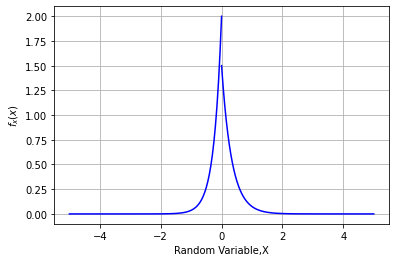
\includegraphics[width=.9\columnwidth] {solutions/ee/2016/33/Assignment_2_Fig_2.png}
    \caption{The PDF of X}
    \label{ee2016-33:fig:The PDF of X}
\end{figure}

The CDF of X is defined as follows:
\begin{align}
    F_X(x)= \pr{X\leq x}
\end{align}
Now for $x<0$,
\begin{align}
\pr{X\leq x} &= \int_{-\infty}^{x}{f_x(x)}\,dx\\
&= \int_{-\infty}^{x}{2e^{4x}}\,dx\\
&= 2\left[\frac{e^{4x}}{4}\right]_{-\infty}^{x}\\
&= 2\left[\frac{e^{4x}}{4}-0\right]\\
&= \frac{e^{4x}}{2}
\end{align}
Similarly for $x\geq0$,
\begin{align}
\pr{X\leq x} &= \int_{-\infty}^{x}{f_x(x)}\,dx\\
&= \int_{-\infty}^{0}{2e^{4x}}\,dx +\int_{0}^{x}{\frac{3}{2}e^{-3x}}\,dx\\
&= 2\left[\frac{e^{4x}}{4}\right]_{-\infty}^{0}+\left[\frac{-e^{-3x}}{2}\right]_{0}^{x}\\
&= 2\left[\frac{1}{4}-0\right]-\frac{1}{2}\left[e^{-3x}-1\right]\\
&= 1-\frac{e^{-3x}}{2}
\end{align}

The CDF of X is as below:
\begin{align}
 F_X(x) = 
  \begin{cases}
  1-\frac{e^{-3x}}{2}, & \text{for } x \geq 0\\
  \frac{e^{4x}}{2}, & \text{for } x < 0
  \end{cases}
\end{align}

The plot for CDF of $X$ can be observed at figure \ref{ee2016-33:fig:The PDF of X}.
\begin{figure}[!ht]
       \centering
    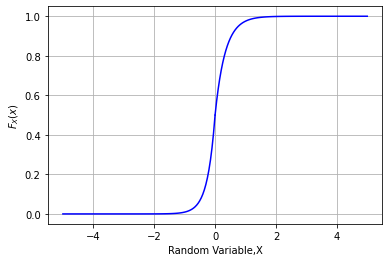
\includegraphics[width=.9\columnwidth] {solutions/ee/2016/33/Assignment_2_Fig_1.png}
    \caption{The CDF of X}
    \label{ee2016-33:fig:The CDF of X}
\end{figure}

\begin{align}
\therefore
\pr{X\leq0} = F_X(0)=\frac{1}{2}
\end{align}




\item A random variable X has probability density function $f(x)$ as given below:\\
\begin{align}
f(x) =
\begin{cases}
a+bx
&  0<x<1
\\      
0
& \text{otherwise}
\end{cases}
\label{a}
\end{align}
\\
If the expected value $E[X]=\dfrac{2}{3}$, then $Pr[X<0.5]$ is..........
\\
\solution

We know that the total probability is one,
\begin{equation}
    \int_{-\infty}^{\infty}{f\brak{x} dx} = 1\label{b}
\end{equation}
Using \eqref{a} in \eqref{b},
\begin{align}
    \int_{0}^{1}{(a+bx)\,dx} = 1\\
    \sbrak{ax+\frac{bx^2}{2}}_0^1=1\\
    \left(a+\frac{b}{2}\right)-0=1\\
    \implies a+\frac{b}{2}=1 \label{c}
\end{align}
We know that expectation value of X,
\begin{align}
    E\brak{X}=\int_{-\infty}^{\infty}xf\brak{x}\,dx\label{d}
\end{align}
%
Using $E\brak{X}=\frac{2}{3}$ and \eqref{a} in \eqref{d}, we get
\begin{align}
     \frac{2}{3}&=\int_{0}^{1}x(a+bx)\,dx\\
     &=\int_{0}^{1} ax+bx^2\,dx\\
     &= \sbrak{\frac{ax^2}{2}+\frac{bx^3}{3}}_0^1\\
     &= \frac{a}{2}+\frac{b}{3}-0\\
     \implies\frac{a}{2}+\frac{b}{3}&=\frac{2}{3}\label{e}
\end{align}
By solving \eqref{c} and \eqref{e}, we get 
\begin{align}
    a\, =\, 0 \,\,and\,\, b\, =\, 2.
\end{align}
Using values of $a$ and $b$ in \eqref{a}, we get
\begin{align}
f\brak{x}
= 
\begin{cases}
2x & 0<x<1
\\
0 & otherwise\label{f}\\
\end{cases}
\end{align}
\begin{figure}[ht]
    \centering
    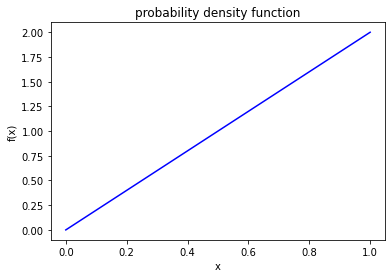
\includegraphics[width=\columnwidth]{solutions/ec/15/figures/assign2.png}
    \caption{Probability Density Function (PDF) of X}
    \label{Figure_1}
\end{figure}
The graph of PDF of X is \ref{Figure_1}
\par Let $F_X(x)$ be the cumulative distribution function of random variable X.
\begin{align}
    F_X(x)=\int_{-\infty}^x f\brak{x} dx\label{x}
\end{align}
$F_X(x)$ can be obtained from the uniform distribution of a random variable U on (0,1) and let U=$X^2$. 
\begin{align}
    0 < U < 1
\end{align}
As for random variable X also,
\begin{align}
    0 < F_X(x) < 1
\end{align}
This similarity between U and $F_X(x)$ is used to generate the random variable X from U.
\begin{align}
    F_X(x)&= \pr{X<x}\\
    &=\pr{\sqrt{U}<x}\\
    &=\pr{U<x^2}\\
    &=F_U(x^2)\label{y}
\end{align}
From uniform distribution,
\\The graph of Probability Density Function (PDF) of U is \ref{Figure_2}
\begin{figure}[ht]
    \centering
    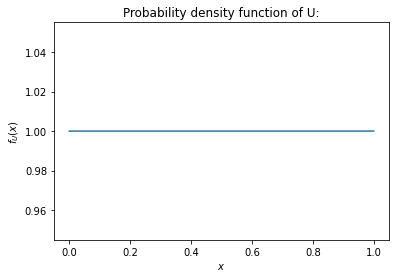
\includegraphics[width=\columnwidth]{solutions/ec/15/figures/assign2_2.png}
    \caption{Probability Density Function (PDF) of U}
    \label{Figure_2}
\end{figure}
\begin{align}
    F_U(x)=
    \begin{cases}
0 & x\leq0\\
x & 0<x<1
\\
1 & x\geq1\label{z}\\
\end{cases}
\end{align}
\begin{figure}[ht]
    \centering
    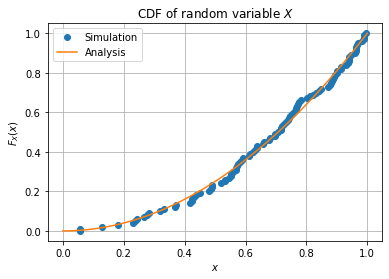
\includegraphics[width=\columnwidth]{solutions/ec/15/figures/assign2_1.png}
    \caption{Cumulative Density Function (CDF)}
    \label{Figure_3}
\end{figure}
\\Using \eqref{z} in \eqref{y},
\\Cumulative distribution function (CDF) of random variable X is,
\begin{align}
F_X(x)= \pr{X<x}
= 
\begin{cases}
0 & x\leq0\\
x^2 & 0<x<1
\\
1 & x\geq1\label{g}\\
\end{cases}
\end{align}
The graph of Cumulative distribution function (CDF) of random variable X is \ref{Figure_3}\\
Now we have to find \pr{X<0.5},Using  \eqref{g},
\begin{align}
    \pr{X<0.5} &= (0.5)^2\\
  \implies \pr{X<0.5} &= 0.25
\end{align}



\item Let X be a random variable with a probability density function
\begin{align}
f(x) = 
\begin{cases}
0.2 & \abs{x}\leq1
\\
0.1 & 1\leq\abs{x}\leq4
\\
0 & otherwise
\end{cases}
\label{pdf}
\end{align}

Find $\pr{0.5< X \leq 5}$
\\
\solution

We know, if X is a continuous random variable, and its p.d.f is given by $f(x)$, then we define the c.d.f $F(x)$ as:
\begin{align}
F(x) = \pr{X \leq x} 
\label{formula1}
\end{align}
and is given by:
\begin{align}
F(x) = \int_{-\infty}^{x}f(x)\,dx 
\label{formula2}
\end{align}

$f(x)$ is a valid p.d.f because: 
\begin{enumerate}
    \item The area under the curve of the p.d.f is 1, i.e:
    \begin{align}
        \int_{-\infty}^{\infty} f(x)\,dx = 1
    \end{align}
    \item $f(x) \geq 0$ for all $x \in \mathbb{R}$\\
\end{enumerate}
Since $f(x)$ is a valid p.d.f, from \eqref{formula2}, we get the following c.d.f:
\begin{align}
F(x) = 
\begin{cases}
0 & x \leq -4
\\
0.1(x + 4) & -4\leq x\leq -1
\\
0.3 + 0.2(x+1) & -1 \leq x \leq 1
\\
0.7 + 0.1(x-1) & 1 \leq x \leq 4
\\
1 & 4 \leq x
\end{cases}
\label{cdf}
\end{align}


    Thus,
    \begin{multline}
    \pr{0.5 \leq X \leq 5} \\ =F(5) - F(0.5) = 0.4
    \end{multline}

\begin{figure}[!ht]
\centering
 \includegraphics[width=\columnwidth]{solutions/ec/20/figures/graph_pdf.png}
 \caption{plot of $f(x)$- p.d.f}
     \includegraphics[width=\columnwidth]{solutions/ec/20/figures/graph_cdf.png}
     \caption{plot of $F(x)$- c.d.f}
 \end{figure}

% The p.d.f is shown below:\\
%  \includegraphics[width=\linewidth]{figures/graph_pdf.png}
% The c.d.f is shown below:\\
%  \includegraphics[width=\linewidth]{figures/graph_cdf.png}



%
\item Consider two identically distributed zero-mean random variables U and V. Let the cumulative distribution functions of U and 2V be F(\textit{x}) and G(\textit{x}) respectively. Then,for all values of \textit{x}
\begin{enumerate}
\begin{multicols}{2}
\setlength\itemsep{2em}
{\small
\item $
F(x)-G(x)\leqslant0
$
\item $
F(x)-G(x)\geqslant0
$
\item $
(F(x)-G(x))\textit{x}\leqslant0
$
\item $
(F(x)-G(x))\textit{x}\geqslant0
$
}
\end{multicols}
\end{enumerate}
%
\solution
If $X$ is a random variable, the cumulative distribution functions of U and 2V can be written in terms of $X$ as
\begin{align} \label{equation-1}
    F(x)=\pr{X \leq x} 
\end{align}
\begin{align}
    G(x)=\pr{2X \leq x}
\end{align}
Or,
\begin{align} \label{equation-2}
     G(x)=\pr{X \leq x/2}
\end{align}
Using \ref{equation-1} in \ref{equation-2}, we can see that
\begin{align} \label{equation-3}
    G(x)=F(x/2)
\end{align}
So,
\begin{align}
    F(x)-G(x)=F(x)-F(x/2)
\end{align}
As F is Cumulative Distribution Function, it is non-decreasing.\\
That means for $x \geq y$, $F(x) \geq F(y)$.\\ \\
Using this, we can form the following table:
\begin{table}[h!]
    \centering
    \begin{tabular}{|c|c|c|}
        \hline
        Case & $F(x)-F(x/2)$ & $(F(x)-F(x/2))x$ \\
        \hline
        $x \geq 0$ & $\geq 0$ & $\geq 0$ \\
        \hline
        $x \leq 0$ & $\leq 0$ & $\geq 0$ \\
        \hline
    \end{tabular}
    \caption{}
    \label{table-1}
\end{table}\\
From the table we can see that for any value of $x$,
\begin{align}
    (F(x)-F(x/2))x \geq 0
\end{align}
Or, using \ref{equation-3},
\begin{align}
    (F(x)-G(x))x \geq x
\end{align}
%
\item A probability density function is of the form\\
{\centering $p(\textit{x}) = Ke^{-\alpha |x|}, \textit{x}\in(-\infty,\infty)$\\}
The value of K is 

\begin{enumerate}
\begin{multicols}{4}
\setlength\itemsep{2em}

\item 0.5
\item 1
\item $0.5\alpha$
\item $\alpha$

\end{multicols}
\end{enumerate}


\item The probability density function (PDF) of a random variable X is as shown in Fig. \ref{fig:2}.
\begin{figure}[!h]
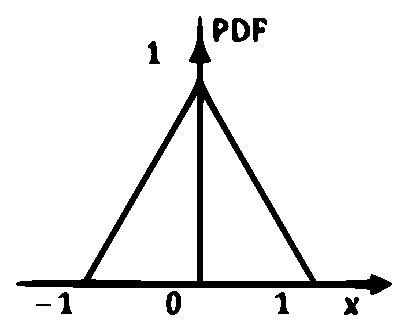
\includegraphics[width=\columnwidth]{./figs/figure2.eps}
\caption{}
\label{fig:2}
\end{figure}

The corresponding cumulative distribution function (CDF) has the form\\

\begin{enumerate}
\begin{multicols}{2}
\setlength\itemsep{4em}

\item Fig. \ref{fig:3}

%\includegraphics{figure3.eps}
\item Fig. \ref{fig:4}

%\includegraphics{figure4.eps}
\item Fig. \ref{fig:5}

% \includegraphics{figure5.eps}
\item Fig. \ref{fig:6}


%\includegraphics{figure6.eps}

\end{multicols}
\end{enumerate}
\begin{figure}[!h]
\includegraphics[width=\columnwidth]{./figs/figure3.eps}
\caption{}
\label{fig:3}
\end{figure}
\begin{figure}[!h]
\includegraphics[width=\columnwidth]{./figs/figure4.eps}
\caption{}
\label{fig:4}
\end{figure}
\begin{figure}[!h]
\includegraphics[width=\columnwidth]{./figs/figure5.eps}
\caption{}
\label{fig:5}
\end{figure}

\begin{figure}[!h]
\includegraphics[width=\columnwidth]{./figs/figure6.eps}
\caption{}
\label{fig:6}
\end{figure}

\item The distribution function $f_x(x)$ of a random variable X is shown in Fig. \ref{fig:12}. The probability that X=1 is
%
\begin{figure}[!h]
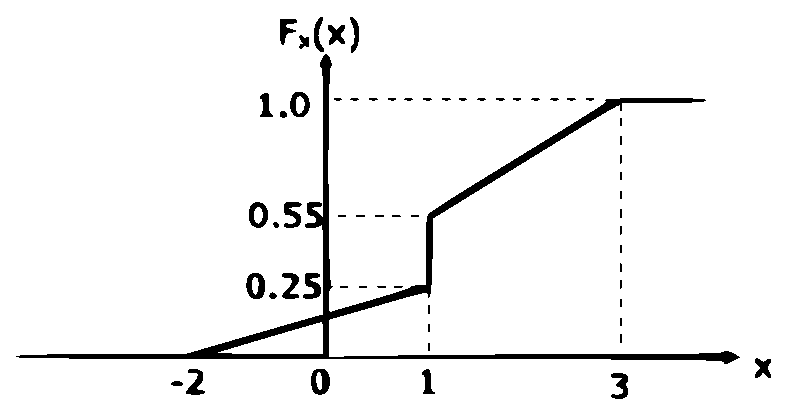
\includegraphics[width=\columnwidth]{./figs/figure12.eps}
\caption{}
\label{fig:12}
\end{figure}


\begin{enumerate}
\begin{multicols}{2}
\setlength\itemsep{1em}

\item Zero
\item 0.25
\item 0.55
\item 0.30

\end{multicols}
\end{enumerate}
%
\item Let the probability density function of a random variable $X$ be 
\begin{center}
$ 
f(x)=
\begin{cases}
x & 0\leq\ x< \frac{1}{2}\\
c(2x-1)^2 &  \frac{1}{2}<x\leq\ 1\\
0 & \text{otherwise}.
\end{cases}
$\\ 
\end{center}


Then,the value of $c$ is equal to \underline{\hspace{3cm}}
\\
\solution
For a probability density function of a continuous random variable, 
\begin{equation}
    \int \limits_{-\infty}^{\infty} f_X(x) \, dx = 1 \label{ec52:eq1}
\end{equation}
\begin{align}
    \int \limits_{-\infty}^{\infty} f_X(x) \, dx &=  \int \limits_0^{1/2} f_X(x) \, dx + \int \limits_{1/2}^1 f_X(x) \, dx\\
    &= \left. \frac{1}{2} (x)(x) \right\rvert_{x = \frac{1}{2}} + \int \limits_{1/2}^1 c(2x-1)^2 \, dx\\
    &= \frac{1}{2}\times\frac{1}{2}\times\frac{1}{2} + c\rsbrak{\brak{\frac{4x^3}{3} - 2x^2 + x}}_{1/2}^1 \\
    &= \frac{1}{8} + c\brak{\frac{1}{3} - \frac{1}{6}} \\
    &= \frac{1}{8} + \frac{c}{6}  \label{ec52:eq6}\\
    \intertext{from \eqref{ec52:eq1}  and \eqref{ec52:eq6} we get }
    1 &= \frac{1}{8} + \frac{c}{6} \\
    \therefore c &= \frac{21}{4}
\end{align}
\begin{figure}[!ht]
\centering
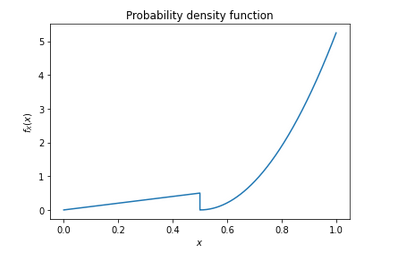
\includegraphics[width=\columnwidth]{solutions/ec/52/figures/pdfimage.png}
\caption{Graph of $f_X(x)$}
\end{figure}
\begin{equation} \label{ec52:eq9}
    F_X(x) = f_X(X<=x) = \int\limits_{-\infty}^x f_X(x) \, dx
\end{equation}
from $f_X(x)$ and equation \eqref{ec52:eq9}, 
\begin{displaymath}
    F_X(x)=\lcbrak{
                    \begin{array}{ll}
                        0 & x\leq 0 \\\\
		                \frac{x^2}{2} &   0 \leq x \leq \frac{1}{2}  \\\\
		                \frac{1}{8} + \frac{7}{8} (2x-1)^3 & \frac{1}{2} \leq x \leq 1 \\\\
		                1 & x>1\\
	                \end{array}    
                }
\end{displaymath}
\begin{figure}[!ht]
\centering
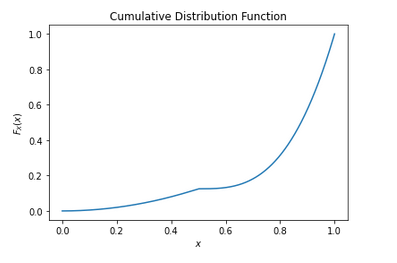
\includegraphics[width=\columnwidth]{solutions/ec/52/figures/cdfimage.png}
\caption{Graph of $F_X(x)$}
\end{figure}



\item Let $X$ be a random variable with the following cumulative distribution function: 

\begin{center}
$ 
F(x)=
\begin{cases}
0 & x<0 \\
x^2 & 0\leq\ x <\frac{1}{2}\\
\frac{3}{4} & \frac{1}{2}\leq\ x<1\\
1 & x\geq\ 1.
\end{cases}
$\\ 

\end{center}
Then $P\brak{\frac{1}{4}<X<1}$ is equal to \underline{\hspace{3cm}}
\\
\solution
\begin{align}
 P ( a \textless x \textless b ) =  F(b) - F(a) \end{align}
We want, 
 \begin{align}
S&= P ( {\dfrac{1}{4}}  \textless  X \textless  1)\\
S&= F(1) - F(\dfrac{1}{4})  \\
S&= \dfrac{3}{4} - \dfrac{1^2}{4^2} \\
S&= \dfrac{11}{16}
\end{align}
Hence, P( ${\frac{1}{4}}$ $ \textless $ X $\textless $ 1) is equal to $\frac{11}{16}$

\begin{figure}[!ht]
\centering
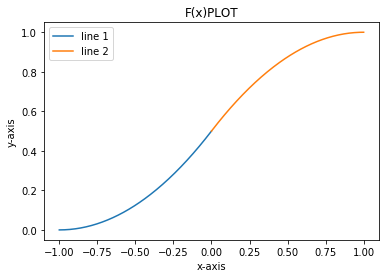
\includegraphics[width=0.5\textwidth]{solutions/ec/54/codes/graph.png}
\label{ec54:fig:graph.png}
\end{figure}






\item Let $X_1$ be an exponential random variable with mean 1 and $X_2$ a gamma random variable with mean 2 and variance 2. If $X_1$ and $X_2$ are independently distributed,then $P(X_1<X_2)$ is equal to \underline{\hspace{3cm}}
\\
\solution
\begin{enumerate}
    \item Given that $X_1$ is an exponential random variable. Let the P.D.F of $X_1$ be
    \begin{align}
    p_{X_1}(x_1)=
        \begin{cases}
        \lambda e^{-\lambda x_1} & x_1 \geq 0\\
        0 & x_1<0
        \end{cases}
    \end{align}
    C.D.F of $x_1$ is :
    \begin{align}
    \begin{split}
        F_{X_1}(x_1)&=\int_{-\infty}^{x_1} p_{X_1}(x_1) dx_1\\
        &=\int_{-\infty}^0 p_{X_1}(x_1) dx_1+\int_{0}^{x_1} p_{X_1}(x_1) dx_1\\
        &=\int_{-\infty}^0 0 \times dx_1+\int_{0}^ {x_1} \lambda e^{-\lambda x_1} dx_1\\
        &=1-e^{-\lambda x_1}\label{ec55:eq:0.0.2}
        \end{split}
    \end{align}
    \begin{align}
    \text{ As mean}=\lambda\\
     \text{ Given that mean}=1\\
     \text{so } \lambda=1 \label{ec55:eq:0.0.5}
    \end{align} 
     
    \item Given that $X_2$ is an gamma random variable.Let the P.D.F of $X_2$ be:
    \begin{align}
        p_{X_2}(x_2)=
        \begin{cases}
            \frac{a^b x_2^{b-1}e^{-ax_2}}{\Gamma(b)} & x_2\geq 0\\
            0 & x_2<0
        \end{cases}\label{ec55:eq:0.0.6}
    \end{align}
    \begin{align}
       \text{ Since mean}=\frac{b}{a}=2\label{ec55:eq:0.0.7}\\
         \text{Also,variance}=\frac{b}{a^2}=2\label{ec55:eq:0.0.8}
    \end{align}
  From \eqref{ec55:eq:0.0.7} and \eqref{ec55:eq:0.0.8}
  \begin{align}
      b=2,a=1\label{ec55:eq:0.0.9}
  \end{align}
  Since the total probability of $X_2$ is 1 \\
  so,\begin{align}
      \int_{-\infty}^\infty p_{X_2}(x_2) dx_2=1
      \end{align}
      \begin{align}
      \int_{-\infty} ^0 p_{X_2}(x_2)
     dx_2+\int_{0}^\infty p_{X_2}(x_2) dx_2&=1\\
      \int_{-\infty} ^0 0\times dx_2+\int_{0}^\infty \frac{a^b x_2^{b-1}e^{-ax_2}}{\Gamma(b)} dx_2&=1
      \end{align}
      \begin{align}
      \frac{a^b}{\Gamma(b)} \int_{0}^\infty x_2^{b-1}e^{-ax_2} dx_2&=1
      \end{align}
      \begin{align}
          \int_{0}^\infty x_2^{b-1}e^{-ax_2} dx_2&=\frac{\Gamma(b)}{a^b}\label{ec55:eq:0.0.14}
  \end{align}
  now substituting $a+\lambda$ for a in \eqref{ec55:eq:0.0.14} gives 
  \begin{align}
      \int_{0}^\infty x_2^{b-1}e^{-(a+\lambda)x_2} dx_2&=\frac{\Gamma(b)}{(a+\lambda)^b}\label{ec55:eq:0.0.15}
  \end{align}
  Now we have to find $P(X_1<X_2)$\\
  \item Given that $X_1$ and $X_2$ are independent random variables,so
  \begin{align}
     P(X_1<X_2|X_2)=F_{X_1}(X_2)=1-e^{-\lambda X_2}\label{ec55:eq:0.0.16}
  \end{align}
  Now,
\begin{align}
      P(X_1<X_2)&=\int_{0}^\infty F_{X_1}(X_2) \times p_{X_2}(x_2)dx_2
      \end{align}
      from \eqref{ec55:eq:0.0.6},\eqref{ec55:eq:0.0.16}
  \begin{align}
     P(X_1<X_2)=\int_{0}^\infty (1-e^{-\lambda X_2})\times \frac{a^b x_2^{b-1}e^{-ax_2}}{\Gamma(b)} dx_2
     \end{align}
     \begin{align}
     P(X_1<X_2)=\frac{a^b}{\Gamma(b)}\int_{0}^\infty x_2^{b-1}(e^{-ax_2}-e^{-(a+\lambda)x_2})dx_2
  \end{align}
      from \eqref{ec55:eq:0.0.14} and \eqref{ec55:eq:0.0.15}
      \begin{align}
     P(X_1<X_2)&=\frac{a^b}{\Gamma(b)}\brak{\frac{\Gamma(b)}{a^b}-\frac{\Gamma(b)}{(a+\lambda)^b}}
     \end{align}
 \begin{align}
      P(X_1<X_2)=1-\frac{a^b}{(a+\lambda)^b}
 \end{align}
 \begin{align}
     P(X_1<X_2)=1-\brak{\frac{a}{a+\lambda}}^b
 \end{align}
 from \eqref{ec55:eq:0.0.5} and \eqref{ec55:eq:0.0.9}
 \begin{align}
     P(X_1<X_2)&=1-\brak{\frac{1}{1+1}}^2\\
     P(X_1<X_2)&=1-\frac{1}{4}=\frac{3}{4}
 \end{align}
\end{enumerate}

\begin{center}
\centering\underline{\textbf{Common Data for the next two Questions :}}
\end{center}

\item 
Let $X$ and $Y$ be jointly distributed random variables such that the conditional distribution of $Y$, given $X$ =$x$, is uniform on the interval $(x-1,x+1)$. Suppose $E(X)=1$ and $Var(X)=\frac{5}{3}$.
\\
The mean of the random variable $Y$ is 
\begin{enumerate}
\begin{multicols}{2}
\setlength\itemsep{2em}

\item $ \frac{1}{2}$\\
\item $1$\\
\item $ \frac{3}{2}$\\
\item $2$

\end{multicols}
\end{enumerate}
\solution
We know that,
\begin{equation}
    f_{Y|X=x}(y)=\frac{f(x,y)}{f_{X}(x)} \label{ec56:eq:2.0.1}
\end{equation}
Given that $f_{Y|X=x}(y)$ is uniform over the interval (x-1,x+1).
\begin{equation}
    \Rightarrow f_{Y|X=x}(y)=
    \begin{cases}
    \frac{1}{2} & y \in \brak{x-1,x+1}\\
    0 & \text{otherwise}
    \end{cases}\label{ec56:eq:2.0.2}
\end{equation}
Given $E(X)=1$
\begin{equation}
    \Rightarrow \int_{-\infty}^{\infty}x f_{X}(x)dx=1 \label{ec56:eq:2.0.3}
\end{equation}
Now consider $E(Y|X=x)$,
\begin{equation}
    E(Y|X=x)=\int_{-\infty}^{\infty}yf_{Y|X=x}(y)dy
\end{equation}
From \eqref{ec56:eq:2.0.2} it simplifies to,
\begin{multline}
    \Rightarrow E(Y|X=x)=\int_{-\infty}^{x-1}yf_{Y|X=x}(y)dy+\\ \int_{x-1}^{x+1}yf_{Y|X=x}(y)dy+\int_{x+1}^{\infty}yf_{Y|X=x}(y)dy
\end{multline}
\begin{align}
    \Rightarrow E(Y|X=x)&=\int_{x-1}^{x+1}y\brak{\frac{1}{2}}dy\\
    &=x
\end{align}
Now we can write ,\\
\begin{align}
    E(Y)&=\int_{-\infty}^{\infty}E(Y|X=x)f_{X}(x)dx\\
    &=\int_{-\infty}^{\infty}xf_{X}(x)dx\\
    &=E(X)
\end{align}
From \eqref{ec56:eq:2.0.3} we get 
\begin{equation}
    E(Y)=1.
\end{equation}
\item The variance of the random variable $Y$ is 
\\
\begin{enumerate}
\begin{multicols}{2}
\setlength\itemsep{2em}

\item $ \frac{1}{2}$\\
\item $ \frac{2}{3}$\\
\item $1$\\
\item $2$

\end{multicols}
\end{enumerate}
\solution
\begin{align}
    Var(Y|X=x)&=\int_{-\infty}^{\infty}(y-E(Y))^2f_{Y|X=x}(y)dy\\
    &=\int_{x-1}^{x+1}(y-1)^2\brak{\frac{1}{2}}dy
\end{align}
\begin{align}
    Var(Y)&=\int_{-\infty}^{\infty}Var(Y|X=x)f_{X}(x)dx\\
    &=\brak{\frac{1}{2}}\int_{x-1}^{x+1}\brak{y^2-2y+1}dy\\
    &=\brak{\frac{1}{2}}\brak{\frac{6x^2+2}{3}+2-4x}\\
    &=x^2-2x+\frac{4}{3}
\end{align}
\begin{align}
  Var(Y)=\int_{-\infty}^{\infty}\brak{x^2-2x+\frac{4}{3}}f_{X}(x)dx\\
   =\int_{-\infty}^{\infty}x^2f_{X}(x)dx-2\int_{-\infty}^{\infty}xf_{X}(x)dx+\\\label{ec57:eq:0.0.19}\frac{4}{3}\int_{-\infty}^{\infty}f_{X}(x)dx\
 \end{align}
\begin{align}
  f_{X}(x)dx=1\\\label{ec57:eq:0.0.20}
 Var(X)=\int_{-\infty}^{\infty}x^2f_{X}(x)dx=\frac{5}{3}\\\label{ec57:eq:0.0.21}
 E(x)=\int_{-\infty}^{\infty}xf_{X}(x)dx=1\\\label{ec57:eq:0.0.22}
 \end{align}
 From \eqref{ec57:eq:0.0.19},\eqref{ec57:eq:0.0.20},\eqref{ec57:eq:0.0.21}and \eqref{ec57:eq:0.0.22} we get
 \begin{align}
     Var(Y)&=\frac{5}{3}-2+\frac{4}{3}\\
     &=1
 \end{align}
\textbf{$\therefore$ Option C is true}

\item Let the random variable $X$ have the distribution function: 
\begin{center}
$ 
F(x)=
\begin{cases}
0 &  \ x<0 \\
\frac{x}{2} &  \ 0\leq\ x <1 \\
\frac{3}{5} &  \ 1\leq\ x<2\\
\frac{1}{2}+\frac{x}{8} &  \ 2\leq\ x<3\\
1 &  \ x\geq\ 3.
\end{cases}
$\\ 
\end{center}

Then $P\brak{2 \leq\ X<4}$ is equal to \underline{\hspace{3cm}}
 \\
\solution

Given F(X) is the CDF of the random variable $X$.
\\$P(2\le X<4)$ will be the sum of all the probabilities of values the random variable $X$ can take in $[2,4)$.
\\So it is the difference between CDF values of the random variable X at X=4- and at X=2-.
\\Therefore,
\begin{align}
P(2\le X<4)&=\lim_{X \to 4-}{F(X)}-\lim_{X \to 2-}{F(X)}
 \\     &= \lim_{X \to 4-}{1}-\lim_{X \to 2-}{\frac{3}{5}}
 \\ &= 1-\frac{3}{5}
 \\ &=\frac{2}{5}=0.4
\end{align}
Hence,$P(2\le X<4) = 0.4$.\begin{figure}[ht]
    \centering
    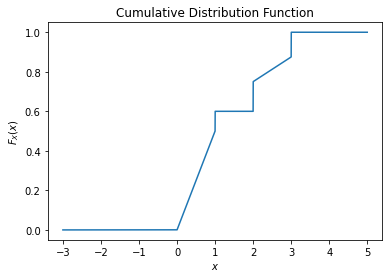
\includegraphics[width=\columnwidth]{solutions/ec/58/CDF.png}
    \caption{CDF of X}
    \label{fig:my_label}
\end{figure}


%
\item Let $X$ be a random variable having the distribution function: 
\begin{center}
$ 
F(x)=
\begin{cases}
0 &  \ x<0 \\
\frac{1}{4} &  \ 0\leq\ x <1 \\
\frac{1}{3} &  \ 1\leq\ x<2\\
\frac{1}{2} &  \ 2\leq\ x<\frac{11}{3}\\
1 &  \ x\geq\ \frac{11}{3}.
\end{cases}
$\\ 
\end{center}

Then $E(X)$ is equal to \underline{\hspace{3cm}}
%
\item Let $\Omega= (0,1]$ be the sample space and let $P(\cdot)$ be a probability function defined by 

\begin{center}
$ 
P((0,x])=
\begin{cases}
\frac{x}{2} &  \ 0 \leq\ x< \frac{1}{2} \\
x &  \  \frac{1}{2} \leq\ x \leq\ 1.
\end{cases}
$\\ 
\end{center}

Then $P\brak{\lbrace\frac{1}{2}\rbrace}$ is equal to \underline{\hspace{3cm}}
%
\item Suppose the random variable $U$ has uniform distribution on $[0,1]$ and $X= -2\log U$. The density of $X$ is

\begin{enumerate}

\item $ 
f(x)=
\begin{cases}
e^{-x} &  \ x>0\\
0 & \text{otherwise}.
\end{cases}
$\\ 

\item $ 
f(x)=
\begin{cases}
2e^{-2x} & \ x>0\\
0 & \text{otherwise}.
\end{cases}
$\\ 

\item $ 
f(x)=
\begin{cases}
\frac{1}{2}e^{-\frac{x}{2}} &  \ x>0\\
0 & \text{otherwise}.
\end{cases}
$\\ 

\item $ 
f(x)=
\begin{cases}
\frac{1}{2} &  \ x \in [0,2]\\
0 & \text{otherwise}.
\end{cases}
$\\ 



\end{enumerate}

\item Suppose $X$ is a real-valued random variable.Which of the following values \textbf{CANNOT} be attained by $E[X]$ and $E[X^2]$, respectively?


\begin{enumerate}
\begin{multicols}{2}
\setlength\itemsep{2em}

\item $
0 \ and \ 1
$
\item $
2  \ and \ 3
$
\item $
\frac{1}{2} \ and \ \frac{1}{3}
$
\item $
2 \ and \ 5
$

\end{multicols}
\end{enumerate}
\solution
We know that
\begin{align}
var(X)&=E[(X-E[X])^2] \label{63:eq:1} \\
var(X)&=E[X^2]-(E[X])^2 \label{63:1}
\end{align}
For uniform distribution in the interval $[a,b]$
\begin{align}
var(X) &= \frac{{(b-a)}^2}{12} \label{63:eq:2}
\end{align}
For uniform distribution,$(b-a)^2 \geq 0$\\
By definition of variance,it is average value of ${(X-E[X])}^2$.\\
Since ${(X-E[X])}^2 \geq 0$ ,average $E[(X-E[X])^2] \geq 0$.
\begin{align}
\therefore var(X) & \geq 0 \label{63:2} \\
\therefore E[X^2]-(E[X])^2 & \geq 0 \label{63:3}
\end{align}
\begin{enumerate}
\item  $E[X]=0$ and $E[X^2]=1$
\begin{align}
E[X^2]-(E[X])^2 &=1 - 0\\
&=1\\
\therefore E[X^2]-(E[X])^2 &\geq 0
\end{align}
$\therefore$ $E[X]=0$ and $E[X^2]=1$ can be attained \\
\item  $E[X]=\frac{1}{2}$ and $E[X^2] =\frac{1}{3}$
\begin{align}
E[X^2]-(E[X])^2 &=\frac{1}{3} - \frac{1}{4}\\
&=\frac{1}{12}\\
\therefore E[X^2]-(E[X])^2 &\geq 0
\end{align}
$\therefore$ $E[X]=\frac{1}{2}$ and $E[X^2]=\frac{1}{3}$ can be attained \\
\item  $E[X]=2$ and $E[X^2]=3$
\begin{align}
E[X^2]-(E[X])^2 &=3 - 4\\
&=-1\\
\therefore E[X^2]-(E[X])^2 &\leq 0
\end{align}
$\therefore$ $E[X]=2$ and $E[X^2]=3$ cannot be attained \\
\item  $E[X]=2$ and $E[X^2]=5$
\begin{align}
E[X^2]-(E[X])^2 &=5 - 4\\
&=1\\
\therefore E[X^2]-(E[X])^2 &\geq 0
\end{align}
$\therefore$ $E[X]=2$ and $E[X^2]=5$ can be attained\\ \\
$\therefore$ $E[X]=2$ and $E[X^2]=3$ cannot be attained\\
\end{enumerate}

\item Let $\Omega = (0,1]$ be the sample space and let $P(.)$ be a probability function defined by \\
$
P((0,x])=
\begin{cases}
\frac{x}{2} 
&  0 \leqslant x < \frac{1}{2} \\
x &  \frac{1}{2} \leqslant x \leqslant 1
\end{cases}
$ \\
Then $P \bigg ( \{ \frac{1}{2} \} \bigg )$ is equal to.......

\item Let X be a random variable with the following cumulative distribution function: \\

$
F(x)= 
\begin{cases}
0 & x<0 \\
x^2 & 0 \leqslant x < \frac{1}{2} \\
\frac{3}{4} & \frac{1}{2} \leqslant x < 1 \\
1 & x \geqslant 1
\end{cases}
$ \\

Then $P({\frac{1}{4}}<x<1)$ is equal to........
\\
\solution

We know that,
\begin{align}
   P\brak{p<X<q} &= F\brak{q^{-}}-F\brak{p} \\
    P\brak{\frac{1}{4} < X < 1} &= F\brak{1^{-}}-F\brak{\frac{1}{4}} \\
    &= \frac{3}{4} - \brak{\frac{1}{4}}^{2}\\
    &= \frac{11}{16}\\
    &= 0.6875
\end{align}
\begin{figure}[!ht]
\centering
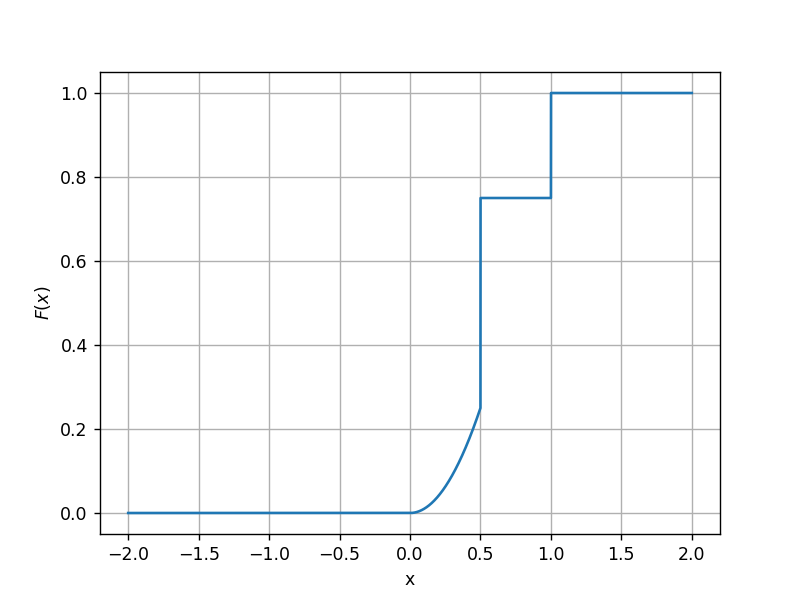
\includegraphics[width=\columnwidth]{solutions/ec/73/Assignment2.png}
\caption{The figure depicts the CDF of X}
\label{ec73:cdf}
\end{figure}



\item Let $X_1$ be an exponential random variable with mean 1 and $X_2$ a gamma random variable with mean 2 and variance 2. If $X_1$ and $X_2$ are independently distributed, then $P(X_1<X_2)$ is equal to.....

\item Suppose the random variable U has uniform distribution on $[0,1]$ and $X= -2 \log U$. The density of X is \\

\begin{enumerate}
\setlength\itemsep{2em}

\item $
f(x)=
\begin{cases}
e^{-x} &  x>0\\
0 & \text{otherwise}
\end{cases}
$

\item $
f(x)=
\begin{cases}
2e^{-2x} &  x>0 \\
0 & \text{otherwise}
\end{cases}
$

\item $
f(x)=
\begin{cases}
\dfrac{1}{2}e^-{\frac{x}{2}} &  x>0 \\
0 & \text{otherwise}
\end{cases}
$

\item $
f(x)=
\begin{cases}
\dfrac{1}{2} &  x \in [0,2] \\
0 & \text{otherwise}
\end{cases}
$

\end{enumerate}
\solution
$U$ - uniformly distributed random variable on $\in$ [0,1]. 
Probability density function of $U$ is: 
\begin{align}
    f_U(u) =
    \begin{cases}
     1  & x \in  [0,1] \\
    0 & \text{otherwise} 
    \end{cases}
\end{align}
 $X$ is given by :
\begin{align}
  X = -2 \ln(U) \\
\implies    0 \leq X \leq \infty
\end{align}
CDF of  $X$ is defined as 
\begin{align}
    F_X(x) &= \pr{X \le x} \\
           &= \pr{-2 \ln(U)\le x} \\
           &= \pr{\ln(U) \ge( -x) /2}\\
           &= \pr {U \ge \exp(-x/2)}\\
           &= 1 - \pr{U \le exp(-x/2)}\\
           &= 1 - exp(-x/2) 
\end{align}
where x $\in$ [0,$\infty$] \\
PDF of $X$ : 
\begin{align}
    f_X(x) & = \frac{d (F_X (x)) }{dx} \\
           & = \frac{1}{2}  exp((-x)/2)
\end{align}
 we have     
\begin{align}
    0 \leq X \leq \infty
\end{align}
\begin{align}
    f_X(x) =
    \begin{cases}
    \frac{1}{2}  exp(\frac{-x}{2}) & x > 0 \\
    0 & \text{otherwise}
    \end{cases}
\end{align}
$\therefore$ answer will be option \brak 3


\item Suppose X is a real-valued random variable. Which of the following values CANNOT be attained by $E[X]$ and $E[X^2]$, respectively?

\begin{enumerate}
\begin{multicols}{2}
\setlength\itemsep{2em}

\item 0 and 1
\item 2 and 3
\item $\dfrac{1}{2}$ and $\dfrac{1}{3}$
\item 2 and 5
\end{multicols}
\end{enumerate}
\solution
The variance of a distribution is given by
\begin{align}
    \sigma^2 %&= \sum_{X \in \mathbb{R}} \left(  (E\left[ X-E[X] \right])^2 \pr{X} \label{varience} \right)\\
    = E[X^2] - E[X]^2
\end{align}
As variance is always positive, 
\begin{align}
    E[X^2] - E[X]^2 \geq 0
\end{align}
is a necessary condition for any real valued random variable. Computing the value of $E[X^2] - E[X]^2$ for the options, we have
\begin{enumerate}[label=(\Alph*)]
\setlength\itemsep{2em}
\item 0 and 1
\begin{align}
    \implies E[X^2] - E[X]^2 = 1 -0^2 = 1 \geq 0
\end{align}
\item 2 and 3
\begin{align}
    \implies E[X^2] - E[X]^2 =3 -2^2 =-1 \leq 0 \label{negative_variance}
\end{align}
\item $\dfrac{1}{2}$ and $\dfrac{1}{3}$
\begin{align}
    \implies E[X^2] - E[X]^2 = \frac{1}{3} - \frac{1}{2}^2 = \frac{1}{12}\geq 0
\end{align}
\item 2 and 5
\begin{align}
    \implies E[X^2] - E[X]^2 = 5 -2^2 = 1 \geq 0
\end{align}
\end{enumerate}

\item Probability density function $p(x)$ of a random variable x is as shown below. The value of $\alpha$ is 

\begin{figure}[!h]
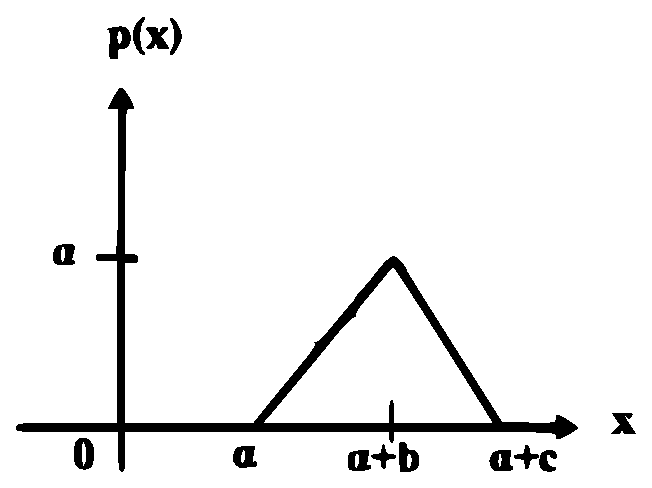
\includegraphics[width=\columnwidth]{./figs/figure13.eps}
\caption{}
\label{fig:13}
\end{figure}


\begin{enumerate}
\begin{multicols}{2}
\setlength\itemsep{2em}

\item $\dfrac{2}{c}$
\item $\dfrac{1}{c}$
\item $\dfrac{2}{(b+c)}$
\item $\dfrac{1}{(b+c)}$

\end{multicols}
\end{enumerate}


%
\item Let the probability density function of random variable,$X$,be given as:\\
\\$f_x(x)$ = $\frac{3}{2}$$e^{-3x}$${u(x)}$ + $a$$e^{4x}$${u(-x)}$\\
\\where u(x) is the unit step function.Then the value of a and Prob\{$X\leq0$\}, respectively,are:\\
\\(A) 2,$\frac{1}{2}$\\
\\(B) 4,$\frac{1}{2}$\\
\\(C) 2,$\frac{1}{4}$\\
\\(D) 4,$\frac{1}{4}$\\
\solution
We know that,
\begin{align}
\int_{-\infty}^{\infty}{f_x(x)}\,dx = 1.\\
\int_{-\infty}^{0}{f_x(x)}\,dx +\int_{0}^{\infty}{f_x(x)}\,dx = 1\label{ee2016-33:eq_(1)}\\
\int_{-\infty}^{0}{ae^{4x}}\,dx +\int_{0}^{\infty}{\frac{3}{2}e^{-3x}}\,dx = 1\label{ee2016-33:eq_(2)}
\end{align}
The expression \eqref{ee2016-33:eq_(2)} was written from \eqref{ee2016-33:eq_(1)} since,
\begin{align*}
  u(x) = 
  \begin{cases}
  1, & \text{for } x \geq 0\\
  0, & \text{otherwise } 
  \end{cases}
\end{align*}

Simplifying \eqref{ee2016-33:eq_(2)} we have:
\begin{align}
\int_{-\infty}^{0}{ae^{4x}}\,dx +\int_{0}^{\infty}{\frac{3}{2}e^{-3x}}\,dx = 1\nonumber\\
\implies a\left[\frac{e^{4x}}{4}\right]_{-\infty}^{0} +    \frac{3}{2}\left[\frac{e^{-3x}}{-3}\right]_0^{\infty} = 1\\
\implies a\left[\frac{1}{4}-0\right] - \frac{1}{2}\left[0-1\right] = 1\\
\implies \frac{a}{4} + \frac{1}{2} =1 \implies a = 2
\end{align}
Therefore,
\begin{align}
 f_x(x) = 
  \begin{cases}
  \frac{3}{2}e^{-3x}, & \text{for } x \geq 0\\
  2e^{4x}, & \text{for } x < 0
  \end{cases}
\end{align}

The plot for PDF of $X$ can be observed at figure \ref{ee2016-33:fig:The PDF of X}
\begin{figure}[!ht]
       \centering
    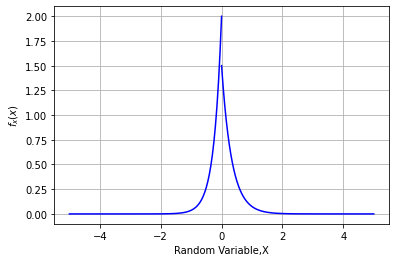
\includegraphics[width=.9\columnwidth] {solutions/ee/2016/33/Assignment_2_Fig_2.png}
    \caption{The PDF of X}
    \label{ee2016-33:fig:The PDF of X}
\end{figure}

The CDF of X is defined as follows:
\begin{align}
    F_X(x)= \pr{X\leq x}
\end{align}
Now for $x<0$,
\begin{align}
\pr{X\leq x} &= \int_{-\infty}^{x}{f_x(x)}\,dx\\
&= \int_{-\infty}^{x}{2e^{4x}}\,dx\\
&= 2\left[\frac{e^{4x}}{4}\right]_{-\infty}^{x}\\
&= 2\left[\frac{e^{4x}}{4}-0\right]\\
&= \frac{e^{4x}}{2}
\end{align}
Similarly for $x\geq0$,
\begin{align}
\pr{X\leq x} &= \int_{-\infty}^{x}{f_x(x)}\,dx\\
&= \int_{-\infty}^{0}{2e^{4x}}\,dx +\int_{0}^{x}{\frac{3}{2}e^{-3x}}\,dx\\
&= 2\left[\frac{e^{4x}}{4}\right]_{-\infty}^{0}+\left[\frac{-e^{-3x}}{2}\right]_{0}^{x}\\
&= 2\left[\frac{1}{4}-0\right]-\frac{1}{2}\left[e^{-3x}-1\right]\\
&= 1-\frac{e^{-3x}}{2}
\end{align}

The CDF of X is as below:
\begin{align}
 F_X(x) = 
  \begin{cases}
  1-\frac{e^{-3x}}{2}, & \text{for } x \geq 0\\
  \frac{e^{4x}}{2}, & \text{for } x < 0
  \end{cases}
\end{align}

The plot for CDF of $X$ can be observed at figure \ref{ee2016-33:fig:The PDF of X}.
\begin{figure}[!ht]
       \centering
    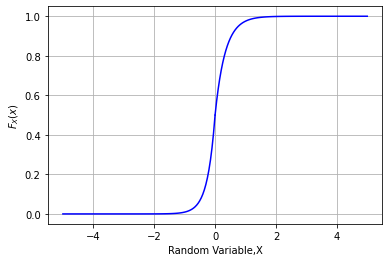
\includegraphics[width=.9\columnwidth] {solutions/ee/2016/33/Assignment_2_Fig_1.png}
    \caption{The CDF of X}
    \label{ee2016-33:fig:The CDF of X}
\end{figure}

\begin{align}
\therefore
\pr{X\leq0} = F_X(0)=\frac{1}{2}
\end{align}




%
\item Suppose $X_i$ for $i = 1, 2, 3$ are independent
and identically distributed random variables
whose probability mass functions are
$\pr{X_i = 0} = \pr{X_i = 1} = \frac{1}{2}$ for $i = 1, 2, 3$.
Define another random variable $Y = X_1 X_2 \oplus X_3$, where $\oplus$ denotes XOR. Then $\pr{Y = 0|X_3 = 0} =$
\\
\solution 

For
\begin{align}
    \because Y = (X_1X_2) \oplus X_3 &= 0\\
    \implies X_1X_2 &= X_3 \label{cs2015-37:all_equal}
\end{align}
\begin{align}
    \pr{Y=0|X_3=0} &= \dfrac{\pr{Y=0,X_3=0}}{\pr{X_3=0}} \label{cs2015-37:eq:0.0.1}\\
    &=\dfrac{\pr{X_1X_2 = X_3, X_3 = 0}}{\pr{X_3=0}}\\
    \pr{X_3 = 0} &= \frac{1}{2} \label{cs2015-37:eq:0.0.2}
\end{align}
if $X_3 = 0$, from \eqref{cs2015-37:all_equal}
\begin{align}
    X_1X_2 &= 0
\end{align}
%The number of possibilities for $X_1X_2=0$
%\begin{align}
%    (X_1,X_2) = \begin{cases}
%(0,0)\\(0,1)\\(1,0)
%\end{cases}
%\end{align}
The random variables are independent of each other:
%\begin{align}
%    \pr{X_i = a, X_j = b} &= \pr{X_i=a} \cdot \pr{X_j=b}\\
%    i \neq j,\quad i,j &\in \{1,2,3\}\\
%    a,b &\in \{0,1\}
%\end{align}
\begin{table}[h!]
    \centering
    \resizebox{\columnwidth}{!}
    {
    \begin{tabular}{|c|c|c|}
    \hline
         $\pr{X_1=0,X_2=0}$& $\pr{X_1=0}\cdot\pr{X_2=0}$&$0.25 $\\ \hline
         
         $\pr{X_1=1,X_2=0}$&$\pr{X_1=1}\cdot\pr{X_2=0}$&$0.25$ \\  \hline
         $\pr{X_1=0,X_2=1}$&$\pr{X_1=0}\cdot\pr{X_2=1}$&$0.25$\\
         \hline
    \end{tabular}
    }
    
    \caption{Probabilities }
    \label{cs2015-37:tab:my_label}
\end{table}
\begin{align}
\nonumber
\pr{X_1X_2=0} &= \pr{X_1=0,X_2=0} \\ \nonumber
    &\quad+ \pr{X_1=0,X_2=1}\\ &\quad+ \pr{X_1=1,X_2=0}\\
    &=\frac{1}{4} +\frac{1}{4} + \frac{1}{4}= \frac{3}{4} 
\end{align}
\begin{align}
    \pr{Y=0,X_3=0} &= \pr{X_1X_2=X_3=0}\\
    &= \pr{X_1X_2=0}\cdot\pr{X_3=0}\\
    &=\frac{3}{4} \cdot \frac{1}{2}\\
    &=\frac{3}{8} \label{cs2015-37:case_A}
\end{align}
Upon substituting \eqref{cs2015-37:case_A} and \eqref{cs2015-37:eq:0.0.2} in \eqref{cs2015-37:eq:0.0.1}
\begin{align}
    \pr{Y=0|X_3=0} = \dfrac{3}{4} = 0.75
\end{align}

%
\item A continuous random variable X has a probability density function 
\begin{align}
 \fn{x} = e^{-x}, \text{where, } 0<x<\infty.
\end{align}
Then \pr{X > 1} is ?
\solution

x is uniform with 
\begin{align}
    0<x<\infty.  
\end{align}
\begin{align}
    \fn{x} = e^{-x} \text{ is uniform, with } 0<\fn{x}<1.
\end{align}
Let, 
\begin{align}
    F_X\brak{x} \text{ be the cumulative distribution function of X.}
\end{align}
\begin{align}
    \text{As, }0<x<\infty, F_X(x) = 0 \text{ for } x<0 
\end{align}
\begin{align}
    F_X\brak{x} &= \pr{X \leq x} = \int_{0}^{x} \fn{x} dx = \int_{0}^{x} e^{-x} dx
    \\&=\sbrak{-e^{-x}}_{0}^{x} = \brak{-e^{-x}} - \brak{-e^{0}} = 1-e^{-x}
    \\\pr{X > 1} &= 1 - F_X\brak{1}
    \\&= 1 - \brak{1-e^{-1}} = 0.368
\end{align}

%
\item Assume that the duration in minutes of a telephone conversation follows the exponential distribution f(x) = $\frac{1}{5}e^{-\frac{x}{5}}$, x $\ge$ 0. The probability that the conversation will exceed five minutes is...
\begin{enumerate}
\item $\frac{1}{e}$ 
\item 1 - $\frac{1}{e}$ 
\item $\frac{1}{e^2}$ 
\item 1 - $\frac{1}{e^2}$
\end{enumerate}
%
%
\solution

Let X be a Random variable defined,that denotes the duration of a telephonic conversation in minutes.\\
So, X $\in$ [0,$\infty$) \\
Given, f$_X$(x) = $\frac{1}{5}e^{-\frac{x}{5}}$ \\
Let CDF of X be F$_X$(x)
\begin{align*}
F_X(x) &=  \int_{-\infty}^{x}f_X(t) \,dt \\
       &= \int_{-\infty}^{0}f_X(t) \,dt + \int_{0}^{x}f_X(t) \,dt \\
F_X(x) &= \int_{0}^{x}f_X(t) \,dt  \because f_X(x) = 0 \forall x<0  \\
\therefore F_X(x) &= \int_{0}^{x}\frac{1}{5}e^{-\frac{t}{5}} \,dt \\
\tag{1}
\label{in2007-27:CDF}
\implies F_X(x) &= 1 - e^{-\frac{x}{5}}
\end{align*}
\begin{align*}
F_X(x) &= \pr{X \le x} \\
\pr{X > 5} &= 1 - \pr{X \le 5} \\
\implies \pr{X > 5} &= 1 - F_X(5) \\
 &= 1 - (1 - e^{-\frac{5}{5}}) \\
 &= e^{-\frac{5}{5}}  \\
 &= e^{-1} = \frac{1}{e}
\end{align*}

%
\item Suppose $Y$ is distributed uniformly in the open interval (1,6). The probability that the polynomial 3$x^2$+6$xY$+3$Y$+6 has only real roots is (rounded off to 1 decimal place) 
%
\solution
 Given, $Y$ has a uniform distribution in the interval (1,6).  
This implies, the probability density function of $Y$,
\begin{align}
f\brak{y} 
= 
\begin{cases}
\frac{1}{6-1} = \frac{1}{5}           & (1<y<6) \\
0           & $otherwise$ 
\end{cases}
\end{align}
 
From this, cumulative distribution function of $Y$, 
\begin{align}
F_Y\brak{y} 
= 
\begin{cases}
\frac{y-1}{5}           & (1<y<6) \\
0           & y \leq 1 \\
1           & y \geq 6 \\
\end{cases}
\end{align}
  Given polynomial: 3$x^2$+(6$Y)x$+(3$Y$+6)  Comparing it with the form: a$x^2$+b$x$+c 

Here, a=3; b=$6Y$; c=$3Y+6$
 Condition for real roots,
\begin{align}
    b^2 - 4ac \geq 0\\
    (6Y)^2 - 4(3)(3Y+6) \geq 0 \\
    Y^2-Y-2 \geq 0\\
 (Y-2)(Y+1) \geq 0
 \end{align}
 \begin{align}
\therefore  Y \leq -1, &  Y \geq 2
\end{align}
Probability that the given polynomial has real roots is,
\begin{align}
   P\brak{Y \leq -1} + P\brak{Y \geq 2} &= F_Y\brak{-1} + 
       1 - F_Y\brak{2^{-}}\\
      &= 0 + 1 - \brak{\frac{2-1}{5}}\\
    &= 0.8
\end{align}

%
\item Let \(X\) be a continuous random variable denoting the temperature measured. The range of temperature is [0,100] degree Celsius and let probability density function of \(X\) be \(f(x)\)=0.01 for 0 \(\leq X \leq\) 100.\newline
The mean of \(X\) is ?\newline
%
\begin{enumerate}[label=(\Alph*)]
    \item \(2.5\)
    \item \(5.0\)
    \item \(25.0\)
    \item \(50.0\)
\end{enumerate}
%
\solution
Given \(X\) is a continuous random variable.
The probability density function of X is \(f(x)\)

\begin{align}
    f(x) = 
	\begin{cases}
	0.01 &  0 \leq x \leq 100\\ ~\\[-1em]
	0 & \text{otherwise}
	\end{cases}
\end{align}
\begin{flushleft}
Mean of the random variable X is \(\mu\)
\end{flushleft}
\begin{align}
    \mu &= \int\limits_{-\infty}^{\infty} x\,f(x)\,\mathrm{d}x =\displaystyle\int\limits_{0}^{100} x\,(0.01)\,\mathrm{d}x\\\nonumber\\
    &=(0.01)\displaystyle\int\limits_{0}^{100} x\,\mathrm{d}x = (0.01)\;\;\frac{x^2}{2}\bigg\vert_0^{100}\\\nonumber\\
    &=50.0 \text{  degree Celsius}\\\nonumber
\end{align}


%
\item The PDF of a Gaussian random variable X is given by 
P$_{X}(x) = \dfrac{1}{3\sqrt{2\pi}}e^{\dfrac{-(x-4)^{2}}{18}}$.The probability of the event { X = 4} is\\
\begin{enumerate}
    \item  $\dfrac{1}{2}$\\
    \item  $\dfrac{1}{3\sqrt{2\pi}}$\\
    \item  0\\
    \item  $\dfrac{1}{4}$\\
\end{enumerate}
%
\solution
Given PDF function is
\begin{align}
  P_{X}(x) &= \dfrac{1}{3\sqrt{2\pi}}e^{\dfrac{-(x-4)^{2}}{18}}
\end{align}
Since continuous probability functions are defined for an infinite number of points over a continuous interval, the probability at a single point is always zero.
\begin{align}
    \pr{x} &=  \lim_{\delta\to 0} \int_{x}^{x+\delta} \dfrac{1}{3\sqrt{2\pi}}e^{\dfrac{-(x-4)^{2}}{18}} \,dx\\
    &=0
\end{align}
Hence the probability is 0.
%

\item Probability density function $p(x)$ of random variable x is as shown below. The value of a is
\begin{enumerate}[label=\Alph*)]
    \item $\frac{2}{c}$
    \item $\frac{1}{c}$
    \item $\frac{2}{(b+c)}$
    \item $\frac{1}{(b+c)}$
\end{enumerate}
\begin{figure}[!ht]
\centering
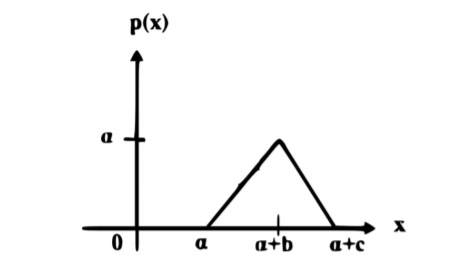
\includegraphics[width=\columnwidth]{solutions/in/2006/2/figures/convolution.png}
\caption{PDF}
\label{in2006-2:fig:convolution}
\end{figure}
%
\solution


Let $Y_1$ and $Y_2$ be two independent and identically distributed (IID) uniform random variables.\\
Let X be a random variable such that
\begin{align}
    X = Y_1 + Y_2
\end{align}
Let
\begin{align}
    p_{Y_1}\brak{y} &= \Pr\brak{Y_1=y} \\
    p_{Y_2}\brak{y} &= \Pr\brak{Y_2=y} \\
    p_X\brak{x} &= \Pr\brak{X=x}
\end{align}
be the probability densities of random variables $Y_1, Y_2$ and $X$. \\
$Y_1$ and $Y_2$ lie in the range \brak{\frac{-c}{4},\frac{c}{4}}, therefore, the PDF for $Y_1$ and $Y_2$,
\begin{align}
p_{Y_1}\brak{y} = p_{Y_2}\brak{y} = 
\begin{cases}
\frac{2}{c} &  \frac{-c}{4} \le y \le \frac{c}{4}\\
0 & \text{otherwise}
\end{cases}
\end{align}

The density of X is obtained by convolution of $Y_1$ and $Y_2$
\begin{align}
p_X\brak{x} = p_{Y_1}(x)*p_{Y_2}(x)
\end{align}
where $*$ denotes the convolution operation. Since convolution operation is time invariant, 
\begin{multline}
    p_X\brak{x-t} = p_{Y_1}(x-t)*p_{Y_2}(x) \\ = p_{Y_1}(x)*p_{Y_2}(x-t)
\end{multline}
On time shifting $Y_1$ by shifting factor $t=a+\frac{c}{2}$, 
\begin{align}
    p_X\brak{x-\brak{a+\frac{c}{2}}} =  p_{Y_1}\brak{x-\brak{a+\frac{c}{2}}}*p_{Y_2}\brak{x}
\end{align}
Thus, the PDF of time shifted X obtained by convolution is,
\begin{align}
p_x = 
\begin{cases}
\frac{4}{c^2}\brak{x-a} & a \le x \le a+\frac{c}{2}\\
\frac{4}{c^2}\brak{a+c-x} & a+\frac{c}{2} \le x \le a+c \\
0 & \text{otherwise}
\end{cases}
\end{align}

On comparing the parameters of PDF of time shifted X with that in the question, we have

\begin{align}
    b=\frac{c}{2}\\
    a=\frac{2}{c}
\end{align}
\rightline{Answer : Option A}


\begin{figure}[!ht]
\centering
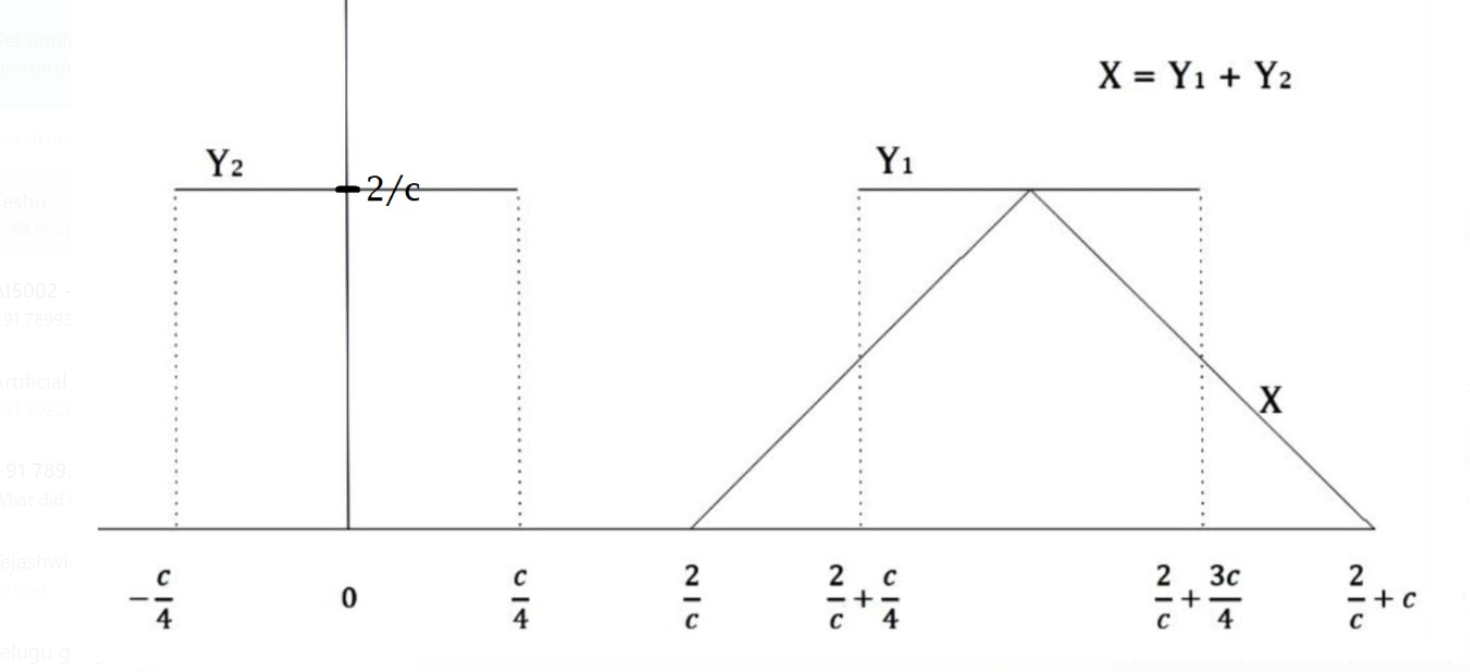
\includegraphics[width=\columnwidth]{solutions/in/2006/2/figures/con6.png}
\caption{PDF of time shifted X}
\label{in2006-2:fig:con6}
\end{figure}
The following are some observations: 
\begin{enumerate}
    \item The sum of two equally distributed random variables will lead to a triangular probability density
    \item The two uniformly distributed random variables lie in the range $\brak{\frac{-c}{4},\frac{c}{4}}$ and $\brak{\frac{2}{c}+\frac{c}{4} , \frac{2}{c}+\frac{3c}{4}}$. \\
     $ \because X = Y_1 + Y_2$ the range of X is thus $\brak{\frac{2}{c},\frac{2}{c}+c}$
    \item On time shifting $Y_1$ to the right by a factor $a+\frac{c}{2}$, the convoluted PDF of X also shifts by the same factor without any change in it's width.
\end{enumerate}

Fig \ref{in2006-2:fig:sim3} and Fig \ref{in2006-2:fig:sim4} are the plots of PDF and CDF obtained by taking c=2
\begin{figure}[!ht]
\centering
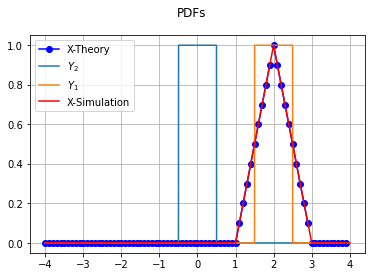
\includegraphics[width=\columnwidth]{solutions/in/2006/2/figures/sim3.png}
\caption{PDF of $Y_1, Y_2$ and X}
\label{in2006-2:fig:sim3}
\end{figure}
\begin{figure}[!ht]
\centering
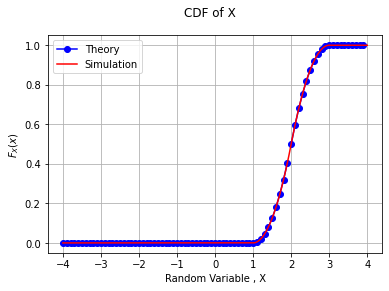
\includegraphics[width=\columnwidth]{solutions/in/2006/2/figures/sim4.png}
\caption{CDF of X}
\label{in2006-2:fig:sim4}
\end{figure}






\end{enumerate}